%% Slides for ".NET Programming" by Chunyu Wang <chunyu@hit.edu.cn> %%

\section{图形界面}

\begin{frame}
\frametitle{.NET 图形界面设计}
\begin{itemize}
\setlength{\itemsep}{8pt plus 1pt}
\item .NET 提供了丰富的类库进行图形界面的设计
\begin{itemize}
\item System.Windows.Forms --- Windows 窗体设计
\item System.Web.UI.WebControls --- Web 表单设计
\item System.Web.UI.MobileControls --- 智能设备窗体的设计
\end{itemize}
\item 各种控件的使用方式灵活,如直接使用或继承后定制
\item 由于 C\# 语言的特点,使图形界面编程非常简单
\item 方便有效的工具,如 Visual Studio 2008 
\end{itemize}
\end{frame}

\begin{frame}
\frametitle{使用控件}
\begin{itemize}
\setlength{\itemsep}{8pt plus 1pt}
\item 图形界面的编程,就是用利用各种控件类的实例
\item 由 CLR 根据控件类型,完成图形界面底层的细节
\item 生成并利用实例的代码,在设计时和运行时是一样的
\item 直接修改控件的特性,即完成控件的设置
\item 对事件的响应,可使用事件句柄或覆盖相应的基类方法
\end{itemize}
\end{frame}

\begin{frame}[fragile]
\frametitle{控件都是类}
\begin{itemize}
\item .NET 中的控件实际就是不同的类
  \begin{itemize}
  \item 窗体类 Form,按钮类 Button,文本框类 TextBox
  \end{itemize}
\item 通过类的成员和方法控制和使用控件
\begin{lstlisting}
using System.Windows.Forms;
using System.Drawing;
...
  TextBox userName = new TextBox();
  
  userName.Name = "InputForUserName";
  userName.Location = new Point(64,88);
  userName.Size = new Size(200,20);
  userName.Text = "Enter your name here!";
\end{lstlisting}
\end{itemize}
\end{frame}

\begin{frame}[fragile]
\frametitle{控件基类(\textit{Control})}
所有的控件都继承自 System.Windows.Forms.Control 类。
\begin{itemize}
\item Control 类主要用于实现控件的基本功能
\item Control 类有 200 多个成员,其中包括各种特性和事件
\item 通过 Control 类,控件之间可以共享相同的行为
\item 也可以通过{\redwarn 覆盖}(\textit{override}),实现自己的不同行为
\end{itemize}
\begin{figure}[htbp]
  \centering
  %% Slides for ".NET Programming" by Chunyu Wang <chunyu@hit.edu.cn> %% $Rev$

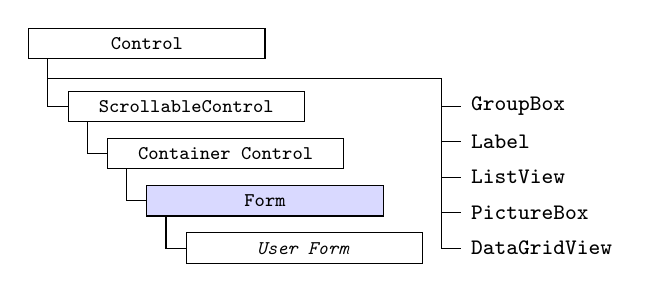
\begin{tikzpicture}
\tikzstyle{every node}=[anchor=west,font=\ttfamily\footnotesize]
\node at (5.5,4.4) (c1) {GroupBox};
\node at (5.5,3.95) (c2) {Label};
\node at (5.5,3.5) (c3) {ListView};
\node at (5.5,3.05) (c4) {PictureBox};
\node at (5.5,2.6) (c5) {DataGridView};

\tikzstyle{every node}=[anchor=west,draw,minimum width=3cm,fill=white,font=\ttfamily\scriptsize]
\node at (0,5.2) (a) {\textbf{Control}};
\node at (.5,4.4) (b) {ScrollableControl};
\node at (1,3.8) (b1) {Container Control};
\node[fill=blue!15] at (1.5,3.2) (b2) {Form};
\node at (2,2.6) (b3) {\textit{User Form}};

\draw (a.south west) +(right:.25cm) |- (b);
\draw (b.south west) +(right:.25cm) |- (b1);
\draw (b1.south west) +(right:.25cm) |- (b2);
\draw (b2.south west) +(right:.25cm) |- (b3);

\draw (.25,4.75) -- (5.25,4.75);

\foreach \a in {c1,c2,c3,c4,c5}
\draw (5.25,4.75) |- (\a);
\end{tikzpicture}

\end{figure}
\end{frame}

\begin{frame}[fragile]
\frametitle{控件的使用方式}
\begin{itemize}
\item 直接使用,通过类库提供的类,生成默认的实例
\item 扩展使用,通过继承类库的类,生成可定制的实例
\end{itemize}
\begin{figure}[htbp]
  \centering
  %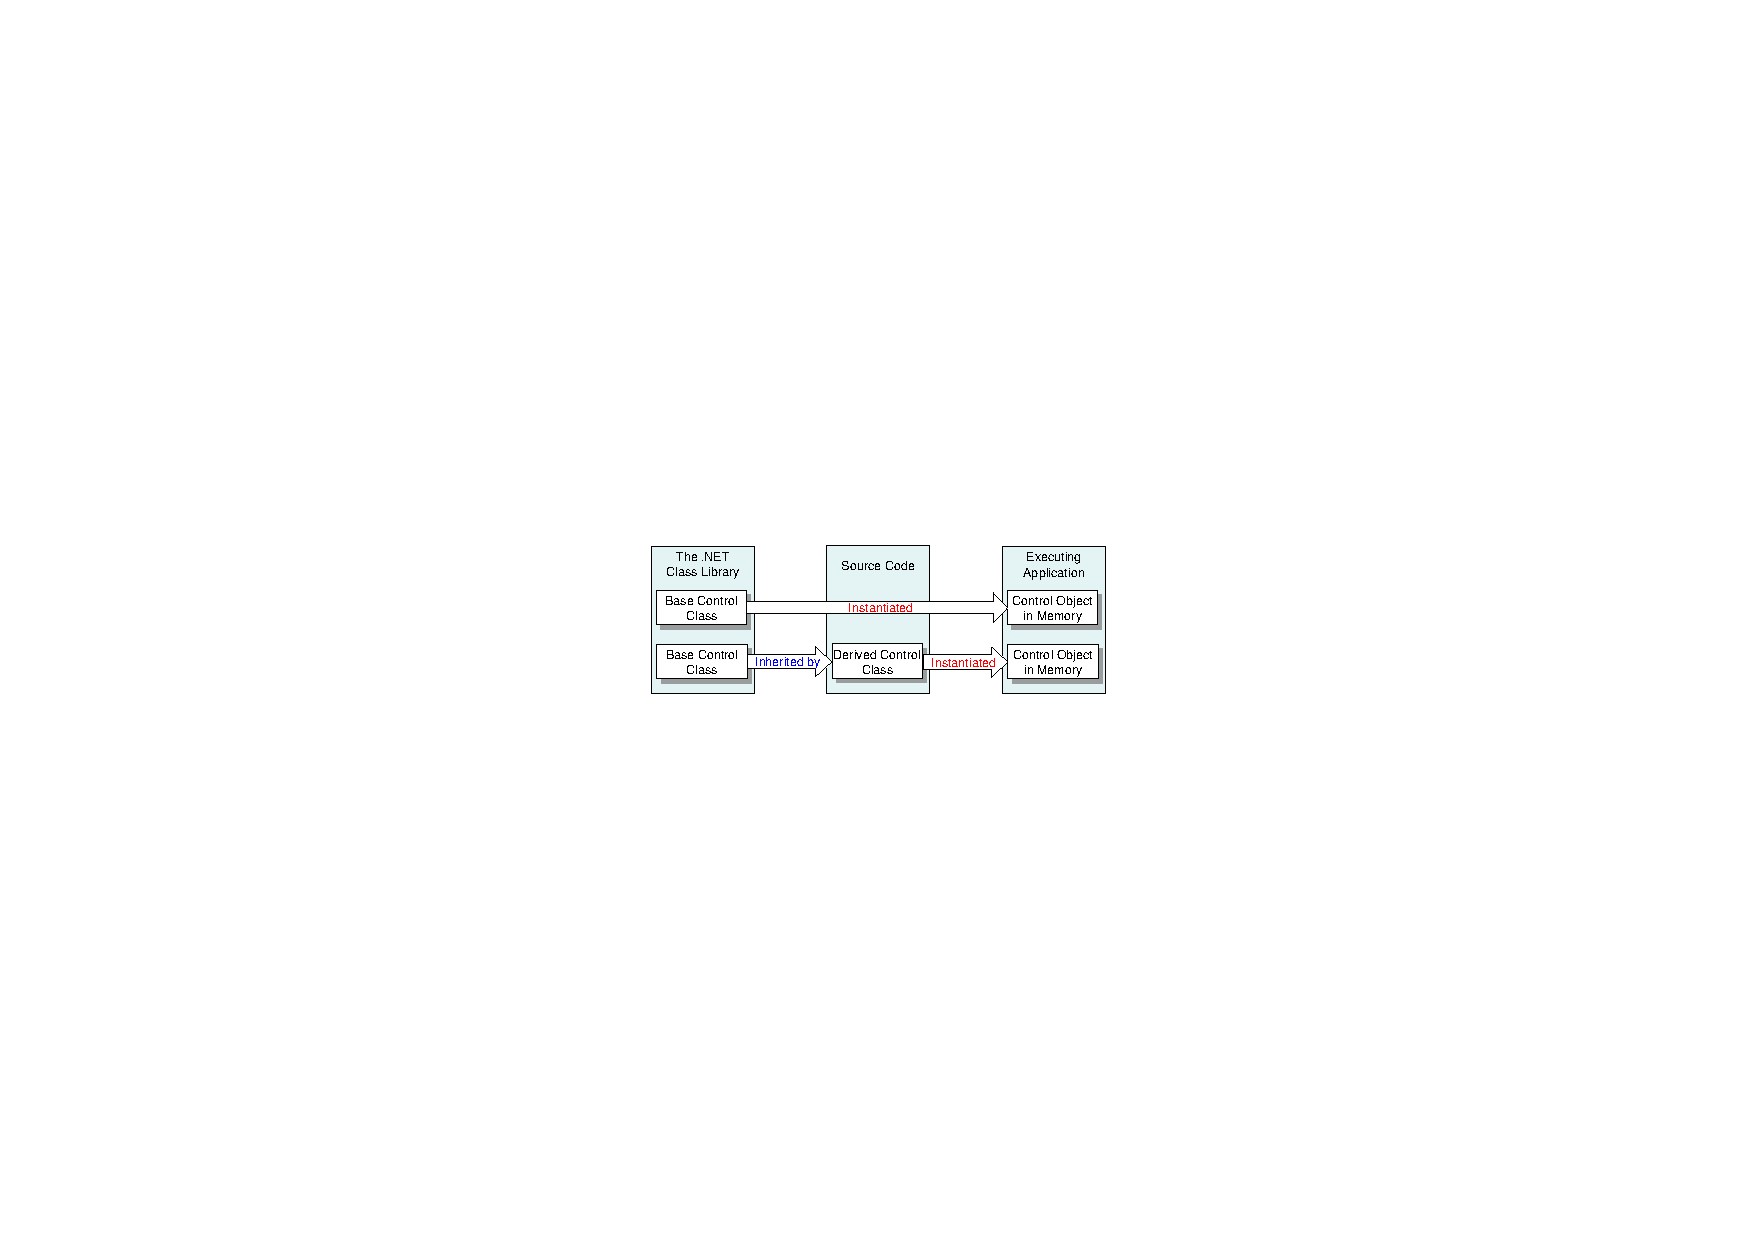
\includegraphics[width=\textwidth, angle=270]{gui-usecontrl}
  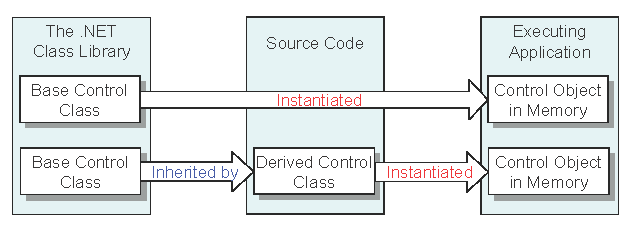
\includegraphics[width=\textwidth]{gui-usecontrl-png}
\end{figure}
\end{frame}

\begin{frame}[fragile]
\frametitle{窗体类(\textit{Form})}
\begin{itemize}
\item 直接使用 Form 类的实例
\item \cmd{csc /t:winexe form.cs}
\end{itemize}
\begin{columns}[t]
\column{.6\textwidth}
\lstset{emph={Form}}
\begin{lstlisting}
// form.cs
using System;
using System.Windows.Forms;
using System.Drawing;

class test
{
  static void Main()
  {
    Form frmMain = new Form();
    frmMain.Text = "Hello World";
    Application.Run(frmMain);
  }
}
\end{lstlisting}
\column{.4\textwidth}
\begin{figure}[htbp]
  \centering
  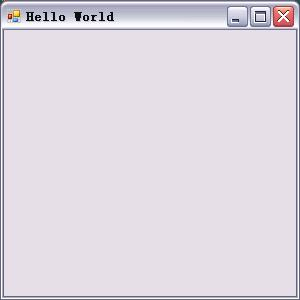
\includegraphics[width=\textwidth]{gui-form1}
\end{figure}
\end{columns}
\end{frame}

\begin{frame}[fragile]
\frametitle{继承窗体类}
\begin{itemize}
\item 通过继承,可以扩展现有控件,自己定制 (\textit{Customize})
\item 例如,派生的 MyForm 窗体,包含一个 TextBox 成员:
\lstset{emph={MyForm}}
\begin{lstlisting}
class MyForm : Form {
  TextBox userName;
  
  public MyForm() // Constructor
  { userName = new TextBox();

    userName.Name = "InputForUserName";
    userName.Location = new Point(64,88);
    userName.Size = new Size(200,20);
    userName.Text = "Enter your name here!";
  }
}
...
  Application.Run(new MyForm());
\end{lstlisting}
\end{itemize}
\end{frame}

\begin{frame}
\frametitle{控件之间的关系}
\begin{itemize}
\item 仅仅作为成员的控件,CLR 无法显示出来
\item 需要将其放入Form 的{\redwarn 控件容器} Controls 中
\item 通过控件容器,实现了控件之间的容纳关系
\end{itemize}
\begin{columns}[t]
  \column{.4\textwidth}
  \begin{figure}[htbp]
    \centering
    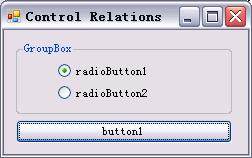
\includegraphics[width=\textwidth]{gui-contains1}
  \end{figure}
  \column{.6\textwidth}
  %% Slides for ".NET Programming" by Chunyu Wang <chunyu@hit.edu.cn> %% -*- coding: utf-8 -*-

\begin{tikzpicture}[font=\sffamily\scriptsize]
\tikzstyle{shnode}=[fill=black!80, fill opacity=.2, minimum width=2.5cm, minimum height=.9cm]
\tikzstyle{outnode}=[fill=red!60!yellow!20, draw=black, fill opacity=.8, minimum width=2.5cm, minimum height=.9cm]
\tikzstyle{innode}=[rounded corners, fill=blue!20, draw=black!40, thin, minimum width=2.4cm, minimum height=.35cm]

\draw \xnode {(3,  4.5)} {a1} {Form Class}        {a11};
\draw \xnode {(1.5,  3)} {b1} {GroupBox Class}    {b11};
\draw \xnode {(4.5,  3)} {b2} {Button Class}      {b21};
\draw \xnode {(.5, 1.5)} {c1} {RadioButton Class} {c11};
\draw \xnode {(3.5,1.5)} {c2} {RadioButton Class} {c21};

\draw[thick] (a11.south) -- ++(down:.35cm) -| (b1.north);
\draw[thick] (a11.south)    ++(down:.35cm) -| (b2.north);
\draw[thick] (b11.south) -- ++(down:.35cm) -| (c1.north);
\draw[thick] (b11.south)    ++(down:.35cm) -| (c2.north);
\end{tikzpicture}

\end{columns}
\end{frame}

\begin{frame}[fragile]
\frametitle{控件容器}
\begin{itemize}
\item System.Windows.Forms.Control.ControlCollection 的实例
\item 实现了 ICollection, IList, IEnumerable 等接口
\item 使用 Add, Remove 的方法,添加、删除控件
\end{itemize}
\begin{lstlisting}
  // init button1 and groupBox1, then 
  this.Controls.Add(this.button1);
  this.Controls.Add(this.groupBox1);

  //init radioButton1 and radioButton2, then
  this.groupBox1.Controls.Add(this.radioButton2);
  this.groupBox1.Controls.Add(this.radioButton1);
\end{lstlisting}
\end{frame}

\begin{frame}[fragile]
\frametitle{访问控件}
\begin{itemize}
\item 使用成员变量,直接访问控件的实例
\item 通过控件的 Controls 容器,逐个遍历
\end{itemize}
\begin{lstlisting}
class MyForm : Form {
  TextBox userName;
  
  public MyForm() // Constructor
  { userName = new TextBox();
    userName.Name = "InputForUserName";
    userName.Location = new Point(64,88);
    userName.Size = new Size(200,20);
    userName.Text = "Enter your name here!";

    this.Controls.Add(userName);
  }
} ...
  Application.Run(new MyForm());
\end{lstlisting}
\end{frame}

\begin{frame}[fragile]
\frametitle{修改控件行为}
\begin{itemize}
\item 修改控件上默认的方法来修改默认行为
\item 扩展的 NumericTextBox 只能输入数字
\end{itemize}
\lstset{emph={override}}
\begin{lstlisting}
public class NumericTextBox : TextBox
{
  protected override void OnKeyPress(KeyPressEventArgs e)
  {
    base.OnKeyPress(e);
    if(!char.IsControl(e.KeyChar) && 
       !char.IsDigit(e.KeyChar)) {
      e.Handled = true;
    }
  }
}
\end{lstlisting}
\end{frame}

\begin{frame}
\frametitle{使用 Visual Studio}
\begin{itemize}
\item 使用 Visual Studio 进行图形界面的设计非常方便
\item 可以通过拖动控件的方式完成设计,修改属性也很方便
\item Visual Studio 中用于图形设计的新项目模板
\begin{itemize}
\item Windows Application
\item Windows Control Library
\end{itemize}
\end{itemize}
\begin{figure}[htbp]
  \centering
  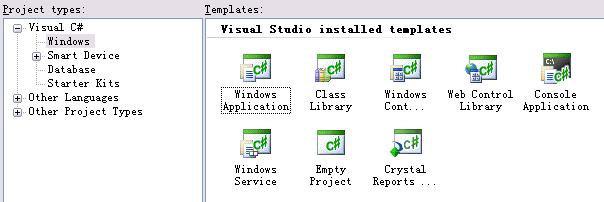
\includegraphics[width=\textwidth]{gui-newproj}
\end{figure}
\end{frame}

\begin{frame}
\frametitle{添加和修改控件}
\begin{itemize}
\item 添加控件只需从工具条拖动到窗口
\item 修改控件,通过特性窗口直接修改
\end{itemize}
\begin{columns}
  \column{.65\textwidth}
  \begin{figure}[htbp]
    \centering
    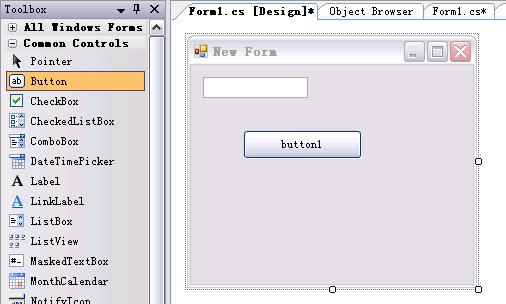
\includegraphics[width=\textwidth]{gui-controls}
  \end{figure}
  \column{.35\textwidth}
  \begin{figure}[htbp]
    \centering
    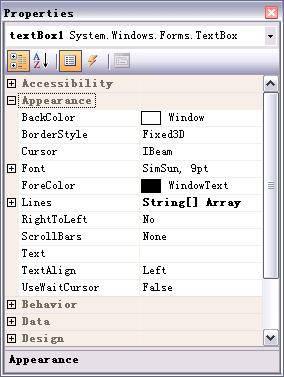
\includegraphics[width=\textwidth]{gui-properties}
  \end{figure}
\end{columns}
\end{frame}

\begin{frame}
\frametitle{智能标签}
\begin{itemize}
\item Visual Studio 还为部分控件提供了智能标签(\textit{Smart Tag})
\item 提供了一些简单任务的快捷方式,直接编辑
\end{itemize}
\begin{figure}[htbp]
  \centering
  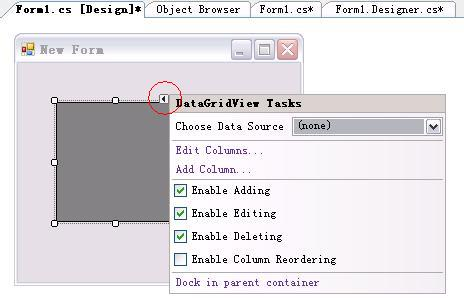
\includegraphics[width=.8\textwidth]{gui-smarttag}
\end{figure}
\end{frame}

\begin{frame}
\frametitle{自动生成的代码}
\begin{itemize}
\item 当创建一个 Windows Application 后,Visual Studio 会自动生成三个源码文件
\begin{itemize}
\item Program.cs --- 程序的入口函数所在文件
\item Form1.Designer.cs --- 主窗口的派生类,及各种控件的初始化
\item Form1.cs --- 主窗口的构造函数
\end{itemize}
\end{itemize}
\begin{figure}[htbp]
  \centering
  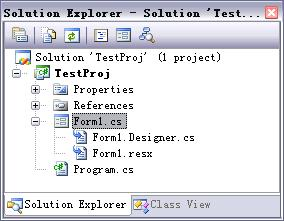
\includegraphics[width=.5\textwidth]{gui-slnwin}
\end{figure}
\end{frame}

\begin{frame}[fragile]
\frametitle{自动生成的组件代码}
\begin{itemize}
\item 使用 InitializeComponent 方法放置组件初始化的代码
\end{itemize}
\lstset{emph={partial,InitializeComponent}}
\begin{lstlisting}
namespace TestWin
{ partial class Form1
  { private System.ComponentModel.IContainer 
      components = null;

    protected override void Dispose(bool disposing)
    { ... }

    private void InitializeComponent()
    { this.components = new 
              System.ComponentModel.Container();
      this.AutoScaleMode = 
              System.Windows.Forms.AutoScaleMode.Font;
      this.Text = "Form1";
    }
  }
}
\end{lstlisting}
\end{frame}

\begin{frame}[fragile]
\frametitle{主函数代码}
\begin{itemize}
\item STAThread 表示线程模式,用于和COM 交互
\item Application.Run() 开始运行标准应用程序消息循环
\end{itemize}
\begin{lstlisting}
[STAThread]
static void Main()
{
  Application.EnableVisualStyles();
  Application.SetCompatibleTextRenderingDefault(false);
  Application.Run(new Form1());
}
\end{lstlisting}
\end{frame}

\begin{frame}[fragile]
\frametitle{窗口的显示}
\begin{itemize}
\item Application.Run 是应用程序入口中标准的显示方法
\item Form.Show() --- 显示窗体,立即返回,主函数继续运行
\item Form.ShowDialog() --- 显示窗体,主函数暂停,等待其退出
\end{itemize}
\begin{columns}
  \column{.5\textwidth}
\begin{lstlisting}
static void Main()
{
  Form m1 = new Form();
  Form m2 = new Form();
  m1.Show();
  m2.Show();
  Thread.Sleep(1000);
}
\end{lstlisting}
  \column{.5\textwidth}
\begin{lstlisting}
static void Main()
{
  Form m1 = new Form();
  Form m2 = new Form();
  m1.ShowDialog();
  m2.ShowDialog();

}

\end{lstlisting}
\end{columns}
\end{frame}

\begin{frame}[fragile]
\frametitle{处理事件 --- 覆盖基类方法}
通过覆盖基类方法,处理事件
\lstset{emph={override}}
\begin{lstlisting}
public class NumericTextBox : TextBox
{
  protected override void OnKeyPress(KeyPressEventArgs e)
  {
    base.OnKeyPress(e);
    if(!char.IsControl(e.KeyChar) && 
       !char.IsDigit(e.KeyChar)) {
      e.Handled = true;
    }
  }
}
\end{lstlisting}
\end{frame}

\begin{frame}[fragile]
\frametitle{处理事件 --- 句柄函数}
使用句柄函数处理事件:
\lstset{emph={Click, clk_handler}}
\begin{lstlisting}
using System;
using System.Windows.Forms;
using System.Drawing;
class test
{ 
  static void Main()
  { Form frmMain = new Form();
    frmMain.Text = "Hello World";

    frmMain.Click += clk_handler;

    Application.Run(frmMain);
  }

  static void clk_handler(object s, EventArgs e)
  {   ((Form)s).Close();     }
}
\end{lstlisting}
\end{frame}

\begin{frame}[fragile]
\frametitle{统一处理事件}
\begin{itemize}
\item 使用句柄函数,可以一处定义,多处使用
\item 提供统一的处理方式
\end{itemize}
\begin{lstlisting}
private void clk_handler(object s, EventArgs e){
  Control ctrl = (Control) s;
  MessageBox.Show("You Clicked: " + ctrl.Name);
}
...
  Button1.Click  += clk_handler;
  TextBox1.Click += clk_handler;
  Label1.Click   += clk_handler;
\end{lstlisting}
\end{frame}


\begin{frame}
\frametitle{常用的控件特性}
\begin{itemize}
\item Control 类提供了大量的特性和事件
\end{itemize}
% \rowcolors[]{1}{blue!20}{blue!10}
\begin{tabular}{l|l}
\hline
特 性                & 说 明                              \\
\hline
Name, Tag            & 名字和相关的数据对象               \\
Controls             & 控件的容器                         \\
Parent               & 所在容器                           \\
\hline
Size, Location       & 控件的大小,位置                   \\
Anchor, Dock         & 控件锚定和停靠的方向               \\
BackColor, ForeColor & 前景色和背景色                     \\
\hline
Text                 & 控件相关的文本,如标题、按钮文字等 \\
Font                 & 默认的字体                         \\
\hline
TabIndex, TabStop    & 按 TAB 建的顺序和焦点             \\
MouseButton          & 鼠标的按键                         \\
MousePosition        & 鼠标的位置                         \\
Cursor               & 光标的形状                         \\
\hline
\end{tabular}
\end{frame}

\begin{frame}[fragile]
\frametitle{使用举例}
\begin{itemize}
\item 控件的停靠 (\textit{Dock})
\begin{lstlisting}
TextBox1.Dock = DockStyle.Top;
\end{lstlisting}
\item 控件的锚定 (\textit{Anchor})
\begin{lstlisting}
Pnl.Anchor = (AnchorStyle.Bottom|AnchorStyle.Left);
\end{lstlisting}
\item 设置 TAB 键顺序
\begin{lstlisting}
TextBox1.TabIndex = 1;
Button1.TabIndex  = 2;
TextBox2.TabIndex = 3;
Button2.TabIndex  = 4;
\end{lstlisting}
\end{itemize}
\end{frame}

\begin{frame}
\frametitle{常用的控件方法}
\begin{figure}
  \centering
  \begin{tabular}{l|l}
    \hline
    方 法        & 说 明                \\
    \hline
    Focus()      & 获取焦点             \\
    DoDragDrop() & 开始拖放操作         \\
    Hide()       & 对用户隐藏控件       \\
    \hline
    Contains()   & 判断是否为控件       \\
    Dispose()    & 释放所有资源         \\
    Scale()      & 缩放控件和任何子控件 \\
    \hline
    OnClick()    & 引发Click事件       \\
    OnEnter()    & 引发Enter事件       \\
    \hline
  \end{tabular}
\end{figure}
\end{frame}

\begin{frame}[fragile]
\frametitle{常用的控件事件}
\begin{itemize}
\item 事件的委托类型
\end{itemize}
\lstset{emph={EventArgs}}
\begin{lstlisting}
delegate void EventHandler(object sender, EventArgs e)
\end{lstlisting}
其中的\texttt{EventArgs} 对不同的事件稍有不同:
\begin{figure}[htbp]
  \centering
  \begin{tabular}{l|l}
    \hline
    事件                   & 事件参数          \\
    \hline
    Click, DoubleClick     & EventArgs         \\
    MouseEnter, MouseLeave & EventArgs         \\
    MouseHover, MouseWheel & EventArgs         \\
    MouseDown, MouseUp     & MouseEventArgs    \\
    KeyUp, KeyDown         & KeyEventArgs      \\
    KeyPress               & KeyPressEventArgs \\
    \hline
  \end{tabular}
\end{figure}
\end{frame}

\begin{frame}
\frametitle{EventArgs 类}
\begin{itemize}
\item EventArgs 类是事件数据类的基类
\item .NET 推荐使用的事件处理参数
\item 利用系统提供的派生类,可以得到事件的信息
\end{itemize}
\medskip

例如,MouseEventArgs 的成员特性:

\begin{tabular}{l|l}
\hline
成员特性 & 说明                                             \\  
\hline
Button   & 枚举MouseButtons 的值Left, Middle, Right, None \\
Clicks   & 鼠标的点击次数                                   \\
Delta    & 鼠标滚轮旋转次数,正数向前,负数向后             \\
X, Y     & 鼠标相对于容器的坐标位置,即控件的 MousePosition \\
\hline
\end{tabular}
\end{frame}

\begin{frame}[fragile]
\frametitle{使用举例}
\begin{itemize}
\item 当鼠标经过时,改变文本框的背景颜色
\end{itemize}
\begin{lstlisting}
  TextBox txtBox = new TextBox(); // and other settings
  txtBox.MouseEnter += OnMouseEnter;
  txtBox.MouseLeave += OnMouseLeave;

void OnMouseEnter(object s, EventArgs e){
  Control ctrl = (Control) s;
  ctrl.BackColor = Color.Red;
}

void OnMouseLeave(object s, EventArgs e){
  Control ctrl = (Control) s;
  ctrl.BackColor = Color.White;
}

\end{lstlisting}
\end{frame}

\begin{frame}
\frametitle{丰富的控件}
\begin{itemize}
\item 类库中的控件种类繁多,十分丰富
\end{itemize}
\begin{figure}[htbp]
  \centering
  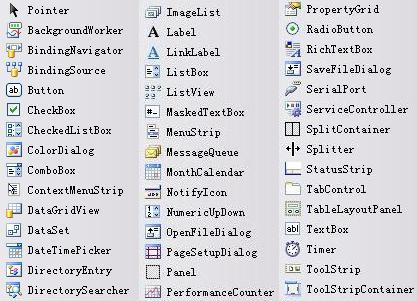
\includegraphics[width=.9\textwidth]{gui-allctrl}
\end{figure}
\end{frame}

\begin{frame}
\frametitle{组件(\textit{Component})}
\begin{itemize}
\item 窗体上除了可以放置控件之外,还可以使用组件
\item 组件就是不可见的控件 (\textit{invisible controls})
\begin{itemize}
\item 显示帮助窗口的组件,系统托盘中显示图标的组件
\item 定时器 Timer,数据库连接 SqlConnection
\end{itemize}
\item 组件和控件的使用基本类似,但不占用窗体空间
\item 在 Visual Studio 中显示在设计窗口之下
\end{itemize}
\begin{figure}[htbp]
  \centering
  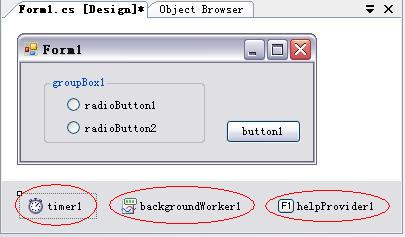
\includegraphics[width=.6\textwidth]{gui-compnts}
\end{figure}
\end{frame}

\begin{frame}[fragile]
\frametitle{组件的使用}
\begin{itemize}
\item Timer 的使用示例
\end{itemize}
\begin{lstlisting}
using System; using System.Windows.Forms;

public class TimerTest {
  static Timer myTimer = new Timer();
  private static void run(object s, EventArgs e) {
    MessageBox.Show ("Hello");
  }
 
  public static void Main() {
    myTimer.Tick += new EventHandler(run);
 
    myTimer.Interval = 1000;
    myTimer.Start();
 
    while(true) Application.DoEvents();
  }
}
\end{lstlisting}
\end{frame}

\begin{frame}[fragile]
\frametitle{组件和控件的区别}
\begin{itemize}
\setlength{\itemsep}{6pt plus 1pt}
\item 一般将组件称为不可见的控件
\item 但实际,控件是组件的一种,控件类继承自组件类
\item 组件不需要放入 Controls 容器中
\item 组件如果使用了非托管的资源,需要显式的释放
\item Visual Studio 会自动分配一个组件容器
\begin{lstlisting}
private
  System.ComponentModel.IContainer components = null;
\end{lstlisting}
\end{itemize}
\end{frame}

% \begin{frame}[fragile]
% \frametitle{窗体类的成员}
% \begin{itemize}
% \item Form 类成员众多,用于设置窗体的各个方面
% \item 成员特性:
% \begin{lstlisting}
% public class Form : ContainerControl{
%   public string Name { get; set; }
%   public Size Size { get; set; }
%   public override string Text { get; set; }
% }
% \end{lstlisting}
% \item 公共方法:
% \begin{lstlisting}
%   public void Activate();
%   public void Close();
% \end{lstlisting}
% \item 可用的事件:
% \begin{lstlisting}
%   public event EventHandler Click;
%   public event EventHandler Activated;
%   public event KeyPressEventHandler KeyPress;
% \end{lstlisting}
% \end{itemize}
% \end{frame}

\begin{frame}[fragile]
\frametitle{MDI 窗体}
\begin{itemize}
\item 实现 MDI (\textit{Multi-Document Interface}) 窗口非常简单
  \begin{itemize}
  \item 设置父窗体的 IsMdiContainer 为 \texttt{true}
  \item 设置子窗体的 MdiParent 为父窗体即可
  \end{itemize}
\end{itemize}
\begin{columns}
  \column{.6\textwidth}
\begin{lstlisting}
Form f1 = new Form();
Form f2 = new Form();

f1.IsMdiContainer = true;
f2.MdiParent = f1;
f2.Show();

Application.Run(f1);
\end{lstlisting}
  \column{.4\textwidth}
  \begin{figure}[htbp]
    \centering
    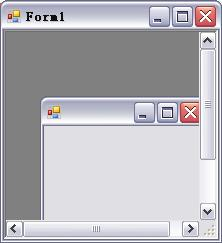
\includegraphics[width=\textwidth]{gui-mdi}
  \end{figure}
\end{columns}
\end{frame}

\begin{frame}[fragile]
\frametitle{菜单的使用}
\begin{columns}
\column{.5\textwidth}
  \begin{itemize}
  \item 将控件 MenuStrip 拖到窗体
  \item 按提示输入想要的菜单项
  \item 选中菜单项,在事件工具栏中选择句柄函数
  \item Visual Studio 自动生成代码
  \end{itemize}
\column{.5\textwidth}
  \begin{figure}[htbp]
    \centering
    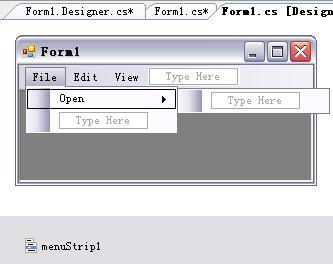
\includegraphics[width=\textwidth]{gui-menu}
  \end{figure}
\end{columns}
\begin{lstlisting}
private MenuStrip menuStrip1;
private ToolStripMenuItem openToolStripMenuItem;
...
openToolStripMenuItem.Size = new Size(152, 22);
openToolStripMenuItem.Text = "Open";
openToolStripMenuItem.Click += 
   new System.EventHandler(this.openToolStripMenuItem_Click);
\end{lstlisting}
\end{frame}

% 具体的控件

% Local Variables:
% mode: LaTeX
% TeX-master: "part-04.tex"
% TeX-header-end: "% End-of-Header$"
% TeX-trailer-start: "% Start-of-Trailer$"
% coding: utf-8
% End:

